% Intended LaTeX compiler: xelatex
\documentclass[10pt, svgnames]{beamer}
\usepackage{graphicx}
\usepackage{longtable}
\usepackage{wrapfig}
\usepackage{rotating}
\usepackage[normalem]{ulem}
\usepackage{amsmath}
\usepackage{amssymb}
\usepackage{capt-of}
\usepackage{hyperref}
\usetheme{focus}
\author{Sappinandana Akamphon}
\date{\today}
\title{Analysis of Multiaxial Stress}
\subtitle{ME 210: Mechanics of Materials}
\usepackage{booktabs}
\usepackage{pgfplots}
\usepackage{amsmath}
\usepackage{bm}
\pgfplotsset{compat=1.18}
\institute{Department of Mechanical Engineering, TSE}
\date{}
\usetikzlibrary{patterns,shapes,arrows}
\setmathfont{Fira Math}
\AtBeginSection[]{\begin{frame}{Outline}\tableofcontents[currentsection]\end{frame}}
\hypersetup{
 pdfauthor={Sappinandana Akamphon},
 pdftitle={Analysis of Multiaxial Stress},
 pdfkeywords={},
 pdfsubject={},
 pdfcreator={Emacs 30.0.50 (Org mode 9.6)}, 
 pdflang={English}}
\usepackage{biblatex}

\begin{document}


\begin{frame}[label={sec:orga0dd01b}]{\{\}}
\maketitle
\end{frame}

\begin{frame}[label={sec:orgbc1b61e}]{Why Should I Care about This?}
\begin{itemize}
\item Many components can be loaded by multiple forces/torques/moments
\item How do we know if material will fail?
\item We need to understand their states of stress first
\begin{itemize}
\item Need to determine max normal and max shear stress
\end{itemize}
\end{itemize}
\end{frame}

\begin{frame}[label={sec:orgd83fa31}]{Determining Max Normal and Shear Stresses}
\begin{itemize}
\item Equivalent normal and shear stresses change with respect to
orientation
\item 2 types of simplification: \emph{plane stress} and \emph{plane strain}
\end{itemize}
\end{frame}

\begin{frame}[label={sec:org7c9ff41}]{Plane Stress: What's That?}
\begin{itemize}
\item Part of material with only \emph{in-plane} normal and shear stresses

\item No stress in \emph{out-of-plane} direction
\end{itemize}

\begin{center}
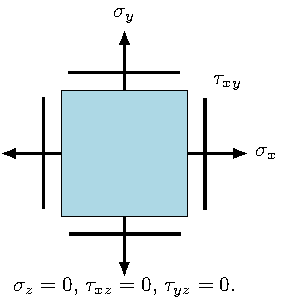
\includegraphics[height=0.7\textheight]{pictures/plane-stress.pdf}
\end{center}
\end{frame}

\begin{frame}[label={sec:orga433dcc}]{Stress Transformation for Plane Stress}
\begin{center}
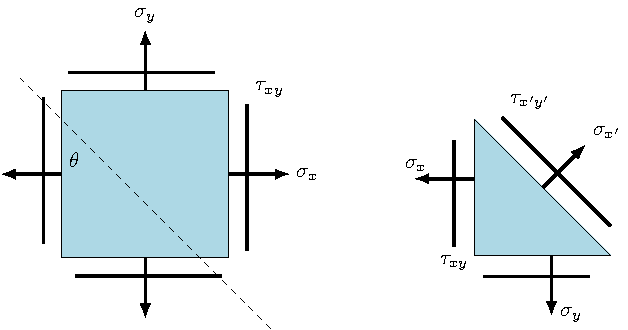
\includegraphics[width=.9\linewidth]{pictures/stress-trans.pdf}
\end{center}

\begin{itemize}
\item Finding maximum normal and shear stresses and their direction

\item Use equilibrium to solve
\end{itemize}
\end{frame}

\begin{frame}[label={sec:org29b0b25}]{Equations for Stress Transformation}
\begin{gather*}
  \sum F_{x'}  = 0; \hfill \\[1em]
  \begin{split}
    \sigma_{x'}\Delta A &- (\tau_{xy}\Delta A\sin \theta )\cos \theta  - (\sigma_y\Delta A\sin \theta )\sin \theta  \\
    &- (\tau_{xy}\Delta A\cos \theta )\sin \theta  - (\sigma_x\Delta A\sin \theta )\cos \theta  = 0
  \end{split} \nonumber \\[0.5em]
  \sigma_{x'} = \sigma_x\cos^2\theta  + \sigma_y\sin^2\theta  + 2\tau_{xy}\sin \theta \cos \theta  \\[1em]
  \sum F_{y'}  = 0; \hfill \\ 
  \tau_{x'y'} = (\sigma_y - \sigma_x)\sin \theta \cos \theta  + \tau_{xy}(\cos^2\theta  - \sin ^2\theta ) \\ 
\end{gather*}

\begin{itemize}
\item \(\sigma_y' = ?\)
\end{itemize}
\end{frame}

\begin{frame}[label={sec:org4073d44}]{Where are My Max Stresses?}
\begin{itemize}
\item Find the max

\[\dfrac{d \sigma_x'}{d\theta} = 0 = - \left( \sigma_x - \sigma_y \right) \sin 2\theta + 2\tau_{xy} \cos 2\theta\]
\[\dfrac{d \sigma_y'}{d\theta} = 0 = \left( \sigma_x - \sigma_y \right) \sin 2\theta - 2\tau_{xy} \cos 2\theta\]

\item For both normal stress in \(x\) and \(y\)
\[2 \theta_p = \tan^{-1} \dfrac{2\tau_{xy}}{\sigma_x - \sigma_y}\]

\item \(\theta_p\) is the \emph{principal direction}
\end{itemize}
\end{frame}

\begin{frame}[label={sec:org3e262d1}]{Graphical Representation of State of Stress}
\begin{itemize}
\item Rewrite stresses using double angle
\end{itemize}

\begin{gather*}
  \sigma_{x'} = \sigma_x\cos^2\theta  + \sigma_y\sin^2\theta  + 2\tau_{xy}\sin \theta \cos \theta  \hfill \\
  \vdots \\
  \sigma_{x'} - \left( \dfrac{\sigma_x + \sigma_y}{2} \right) = \left( \dfrac{\sigma_x + \sigma_y}{2} \right)\cos 2\theta  + {\tau_{xy}}\sin 2\theta  \hfill
\end{gather*}

\begin{gather*}
  \tau_{x'y'} = (\sigma_y - \sigma_x)\sin \theta \cos \theta  + \tau_{xy}(\cos^2\theta  - \sin^2\theta ) \\
  \vdots \\
  \tau_{x'y'} = \left( \dfrac{\sigma_y - \sigma_x}{2} \right)\sin 2\theta  + \tau _{xy}\cos 2\theta \hfill
\end{gather*}
\end{frame}

\begin{frame}[label={sec:org94440c8}]{Getting There\ldots{}}
\begin{itemize}
\item Square both terms and add
\end{itemize}

\begin{align*}
    \Biggl[ \sigma_{x'} -& \left( \dfrac{\sigma_x + \sigma_y}{2} \right) \Biggr]^2 + \tau_{x'y'}^2 = \\
     & \left( \dfrac{\sigma_x - \sigma_y}{2} \right)^2\cos^2 2\theta  + 2\left( \dfrac{\sigma_x - \sigma_y}{2} \right)\tau_{xy}\cos 2\theta \sin 2\theta + \tau_{xy}^2\sin^2 2\theta \\
    +& \left( \dfrac{\sigma_x - \sigma_y}{2} \right)^2 \sin^2 2\theta  + 2\left( \dfrac{\sigma_y - \sigma_x}{2} \right)\tau_{xy}\cos 2\theta \sin 2\theta  + \tau_{xy}^2\cos^2 2\theta
\end{align*}
\end{frame}

\begin{frame}[label={sec:org3c9cf76}]{The Representation}
\begin{itemize}
\item Use trigonometry identities

\[\left[ \sigma_{x'} - \left( \dfrac{\sigma_x + \sigma_y}{2} \right) \right]^2 + \tau_{x'y'}^2 = \left( \dfrac{\sigma_x - \sigma_y}{2} \right)^2 + \tau_{xy}^2\]

\item What shape does that take?
\end{itemize}

\[\left( \sigma_{x'} - \sigma_{avg} \right)^2 + \tau_{x'y'}^2 = R^2\]
\end{frame}

\begin{frame}[label={sec:org3da0ade}]{Mohr's Circle}
\begin{center}
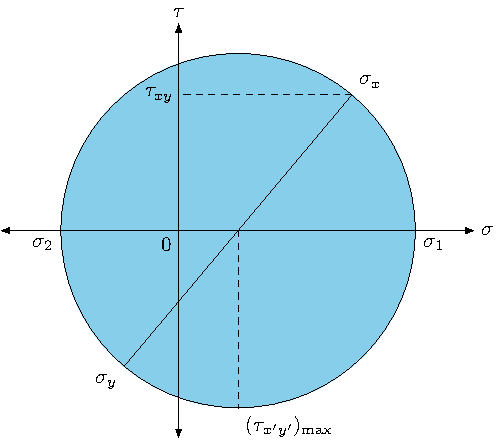
\includegraphics[height=0.9\textheight]{pictures/mohrs-circle.pdf}
\end{center}
\end{frame}

\begin{frame}[label={sec:org2f314de}]{Principal Stresses}
\begin{itemize}
\item Maximum and minimum normal stresses = normal stresses at principal
direction
\end{itemize}

\[\sigma_{x'} (\theta = \theta_p) = \sigma_1 = \dfrac{\sigma_x + \sigma_y}{2} + \sqrt{ \left( \dfrac{\sigma_x - \sigma_y}{2} \right)^2 + \tau_{xy}^2 }\]
\[\sigma_{y'} (\theta = \theta_p) = \sigma_2 = \dfrac{\sigma_x + \sigma_y}{2} - \sqrt{ \left( \dfrac{\sigma_x - \sigma_y}{2} \right)^2 + \tau_{xy}^2 }\]

\begin{itemize}
\item \(\sigma_1\) and \(\sigma_2\) are called \emph{principal stresses}
\end{itemize}
\end{frame}

\begin{frame}[label={sec:orga975a3f}]{Shear Stresses at \(\theta_p\)}
\[\tau_{x'y'} (\theta = \theta_p) = 0\]

\begin{itemize}
\item No shear stress in the principal direction, \emph{ever!}

\item Check on Mohr's circle

\item So where's the maximum shear stress?
\end{itemize}
\end{frame}

\begin{frame}[label={sec:org19359af}]{Maximum In-plane Shear Stress}
\[\dfrac{d\tau_{xy}}{d\theta} = 0 = 2\left( \dfrac{\sigma_y - \sigma_x}{2} \right) \cos 2\theta - 2\tau_{xy} \sin 2\theta\]
\[\tan 2\theta_s = \dfrac{\sigma_y - \sigma_x}{2\tau_{xy}}\]

\begin{itemize}
\item \(\theta_s\) is the maximum shear stress direction
\[\tau_{\max} = \tau_{xy} (\theta = \theta_s)\]

\item \(\tau_{\max}\) is the maximum in-plane shear stress
\end{itemize}
\end{frame}

\begin{frame}[label={sec:org938ef91}]{Example: State of Stress of a Square Element}
\begin{columns}
\begin{column}{0.4\columnwidth}
\begin{center}
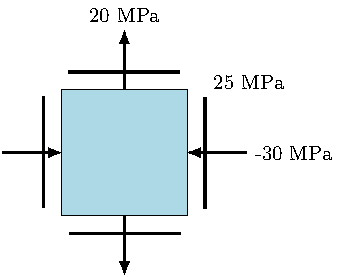
\includegraphics[width=\textwidth]{pictures/example-I-prob.pdf}
\end{center}
\end{column}

\begin{column}{0.6\columnwidth}
\begin{itemize}
\item First, find \(\tau_{\max}\)

\begin{align*}
  \tau_{\max} &= \sqrt {\left( \frac{\sigma_x - \sigma_y}{2} \right)^2 + \tau _{xy}^2}  \\
              &= \sqrt {\left( \frac{-30 - 20}{2} \right)^2 + 25^2}  \\
              &= 35.4 \text{ MPa}
\end{align*}
\end{itemize}
\end{column}
\end{columns}
\end{frame}

\begin{frame}[label={sec:orgc737f95}]{Continue}
\begin{itemize}
\item Principal stresses are

\begin{align*}
  \sigma_{1,2} &= \frac{\sigma_x + \sigma _y}{2} \pm \sqrt {\frac{\sigma _x - \sigma_y}{2}^2 + \tau _{xy}^2}  \\
               &= \frac{-30 + 20}{2} \pm 35.4 \\
               &= 30.4 \text{ MPa}, - 40.4 \text{ MPa}
\end{align*}

\item Principal direction is

\begin{align*}
  2\theta  &= \tan^{-1}\frac{2\tau_{xy}}{\sigma_x - \sigma_y} \\
           &= -45^{\circ} \\
  \theta &= -22.5^{\circ}
\end{align*}
\end{itemize}
\end{frame}

\begin{frame}[label={sec:org0017a3a}]{}
\begin{center}
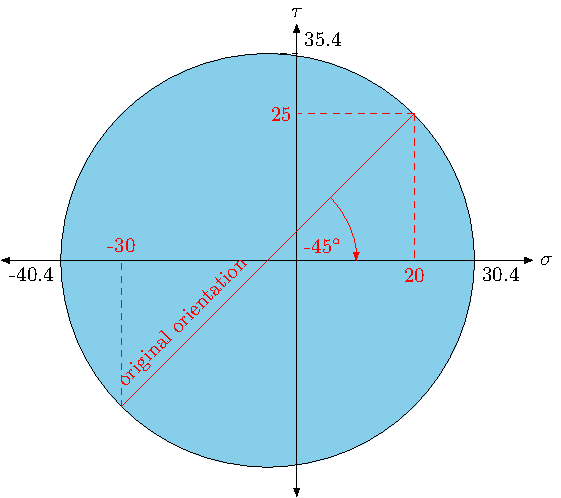
\includegraphics[width=.9\linewidth]{pictures/example-I-mohrs.pdf}
\end{center}
\end{frame}

\begin{frame}[label={sec:orgebaab26}]{Original vs Principal}
\begin{center}
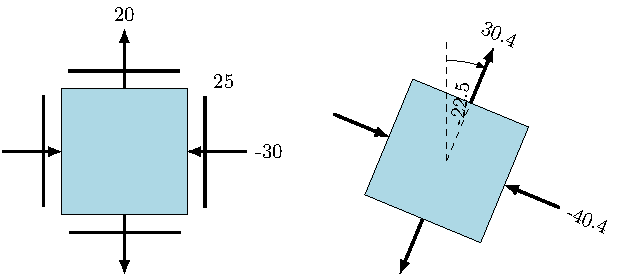
\includegraphics[width=.9\linewidth]{pictures/orig-vs-principal-I.pdf}
\end{center}
\end{frame}

\begin{frame}[label={sec:org6fbd44f}]{Another Example:}
\begin{columns}
\begin{column}{0.4\columnwidth}
\begin{center}
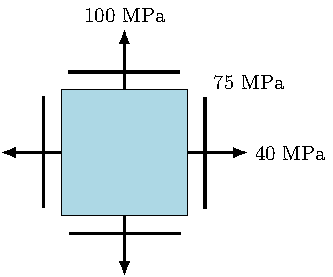
\includegraphics[width=\textwidth]{pictures/example-II-prob.pdf}
\end{center}
\end{column}

\begin{column}{0.6\columnwidth}
\begin{itemize}
\item First, find \(\tau_{\max}\)
\end{itemize}

\begin{align*}
  \tau_{\max} &= \sqrt {\left( \frac{\sigma_x - \sigma_y}{2} \right)^2 + \tau _{xy}^2}  \\
              &= \sqrt {\left( \frac{40 - 100}{2} \right)^2 + 75^2}  \\
              &= 80.8 \text{ MPa}
\end{align*}
\end{column}
\end{columns}
\end{frame}

\begin{frame}[label={sec:orgc502be2}]{Continue}
\begin{itemize}
\item Principal stresses are

\begin{align*}
  \sigma_{1,2} &= \frac{\sigma_x + \sigma _y}{2} \pm \sqrt {\frac{\sigma _x - \sigma_y}{2}^2 + \tau _{xy}^2}  \\
               &= \frac{40 + 100}{2} \pm 80.8 \\
               &= 150.8 \text{ MPa}, - 10.8 \text{ MPa}
\end{align*}

\item Principal direction is

\begin{align*}
  2\theta  &= \tan^{-1}\frac{2(80.8)}{40 - 100} \\
           &= -69.6^{\circ} \\
  \theta &= -34.8^{\circ}
\end{align*}
\end{itemize}
\end{frame}

\begin{frame}[label={sec:org30d12d1}]{}
\begin{center}
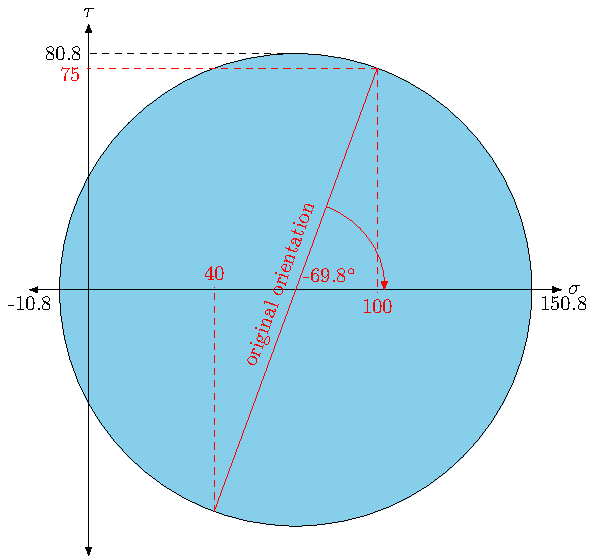
\includegraphics[width=.9\linewidth]{pictures/example-II-mohrs.pdf}
\end{center}
\end{frame}


\begin{frame}[label={sec:org801a719}]{Original vs Principal}
\begin{center}
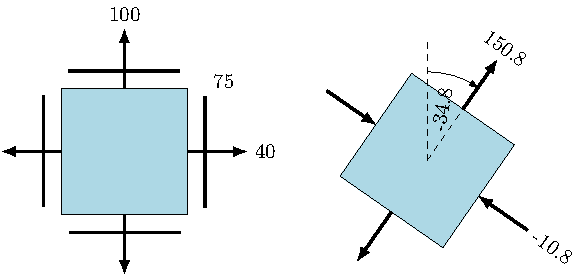
\includegraphics[width=.9\linewidth]{pictures/orig-vs-principal.pdf}
\end{center}
\end{frame}

\begin{frame}[label={sec:orgb8ce6f2}]{Hooke's Law for 3D Stress}
\begin{columns}
\begin{column}{0.4\columnwidth}
\begin{center}
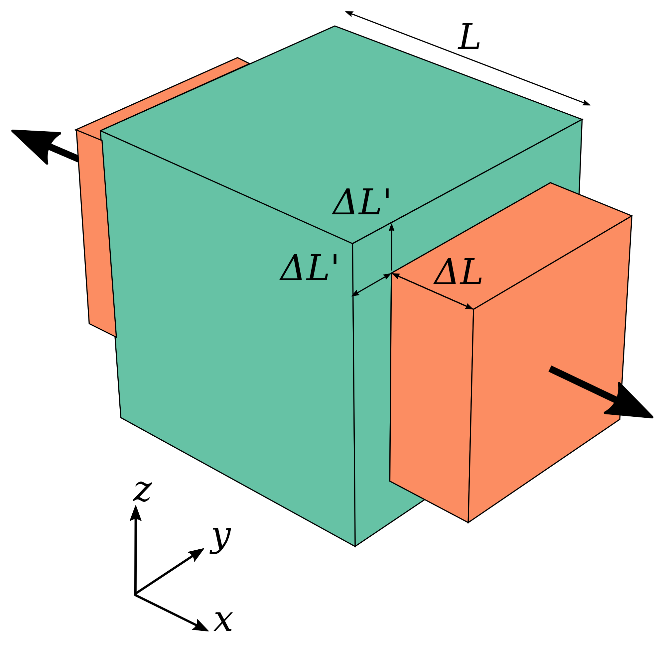
\includegraphics[width=\textwidth]{pictures/3d-poisson.png}
\end{center}
\end{column}

\begin{column}{0.6\columnwidth}
\begin{itemize}
\item Recall Poisson's ratio where
\[\nu = - \dfrac{\varepsilon_{trans}}{\varepsilon_{long}}\]

\item In 3D materials, there are \emph{two} transversal strains

\begin{itemize}
\item For \(x\), there are \(y\) and \(z\)
\end{itemize}
\end{itemize}
\end{column}
\end{columns}
\end{frame}

\begin{frame}[label={sec:orgff20b5b}]{Rethinking Strains in 3D}
\begin{center}
\begin{tabular}{llll}
\toprule
 & \(\sigma_x\) & \(\sigma_y\) & \(\sigma_z\)\\[0pt]
\midrule
\(\varepsilon_x\) & \(\dfrac{\sigma_x}{E}\) & \(-\nu \dfrac{\sigma_y}{E}\) & \(-\nu \dfrac{\sigma_z}{E}\)\\[0pt]
\(\varepsilon_y\) & \(-\nu \dfrac{\sigma_x}{E}\) & \(\dfrac{\sigma_y}{E}\) & \(-\nu \dfrac{\sigma_z}{E}\)\\[0pt]
\(\varepsilon_z\) & \(-\nu \dfrac{\sigma_x}{E}\) & \(-\nu\dfrac{\sigma_y}{E}\) & \(\dfrac{\sigma_z}{E}\)\\[0pt]
\bottomrule
\end{tabular}
\end{center}
\end{frame}

\begin{frame}[label={sec:orgcd32728}]{Volume Change}
\begin{itemize}
\item Original volume of element \(V_0 = abc\)

\item Final volume is

\begin{align*}
  V_{final} &= a \left( 1 + \varepsilon_x \right) b \left( 1 + \varepsilon_y \right) c \left( 1 + \varepsilon_z \right) \\
            &\approx abc \left( 1 + \varepsilon_x + \varepsilon_y + \varepsilon_z \right)
\end{align*}

\item Volume change is
\[V_{final} = abc \left( \varepsilon_x + \varepsilon_y + \varepsilon_z \right)\]
\end{itemize}
\end{frame}

\begin{frame}[label={sec:orgb904a0e}]{Unit Volume Change, \(e\)}
\begin{itemize}
\item Also called \emph{dilatation} or \emph{volumetric strain}
\[e = \frac{\Delta V}{V_0} = \varepsilon_x + \varepsilon_y + \varepsilon_z\]
\end{itemize}
\end{frame}

\begin{frame}[label={sec:org6d5f167}]{Spherical Stress and Bulk Modulus}
\begin{itemize}
\item Spherical stress \(\rightarrow\) same normal stresses in 3 axes
\[\sigma_x = \sigma_y = \sigma_z = \sigma_0\]
\[\varepsilon_x = \varepsilon_y = \varepsilon_z = \frac{1-2\nu}{E} \sigma_0\]
\[e = \frac{3(1-2\nu)}{E} \sigma_0\]

\item Bulk modulus, \(K\), is defined as
\[K = \frac{\sigma_0}{e} = \frac{E}{3(1-2\nu)}\]
\end{itemize}
\end{frame}

\begin{frame}[label={sec:orgae04664}]{Example: Cube under hydrostatic pressure}
A 0.25-m\(^3\) cube is being submerged under water where the water pressure is 30 MPa. If the material has \(E\) = 3 GPa and Poisson's ratio of 0.3, find the final volume of the element.

\begin{center}
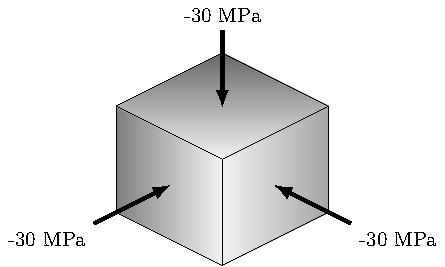
\includegraphics[width=0.6\textwidth]{pictures/cube-under-hydro-pressure.pdf}
\end{center}
\end{frame}

\begin{frame}[label={sec:orgf69a7fd}]{Solution: Cube under hydrostatic pressure}
Hydrostatic pressure situation represents the state where the pressure is equal in all direction. This means that we can assume that the element is under spherical stress. The unit volume change is

\begin{align*}
  e &= \frac{3\sigma_o}{E}(1 - 2\nu ) \\ 
    &= \frac{3(-30 \times 10^6 \text{ Pa})(1 - 2(0.3))}{(3 \times 10^9 \text{ Pa})} \\ 
    &= -0.012 
\end{align*}
\end{frame}

\begin{frame}[label={sec:org9e2727a}]{Solution: Cube under hydrostatic pressure}
This means that the volume reduced by 1.2\% (since hydrostatic pressure in this case is compressive), and thus the final volume is

\begin{align*}
  V_f &= (1 + e)V \\ 
      &= 0.988(0.25 \text{ m}^3) \\ 
      &= 0.247 \text{ m}^3
\end{align*}
\end{frame}

\begin{frame}[label={sec:orgb83a54c}]{Absolute Maximum Shear Stress}
\begin{itemize}
\item In 3D plane stress problems, there are 3 principal stresses.

\item The 3rd principal stress is 0.

\item Use Mohr's circle to represent the relationship of all three.

\item 2 cases:

\begin{enumerate}
\item \(\sigma_1, \sigma_2 > 0\)

\item \(\sigma_1 > 0, \sigma_2 < 0\)
\end{enumerate}
\end{itemize}
\end{frame}

\begin{frame}[label={sec:org29564c2}]{Case I: Stresses are of the Same Sign}
\begin{center}
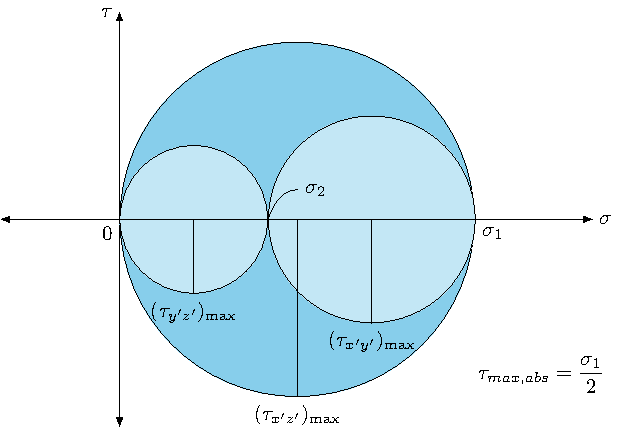
\includegraphics[width=.9\linewidth]{pictures/abs-max-shear-case-I.pdf}
\end{center}
\end{frame}

\begin{frame}[label={sec:org8983b0d}]{Case II: Stresses are of Opposite Signs}
\begin{center}
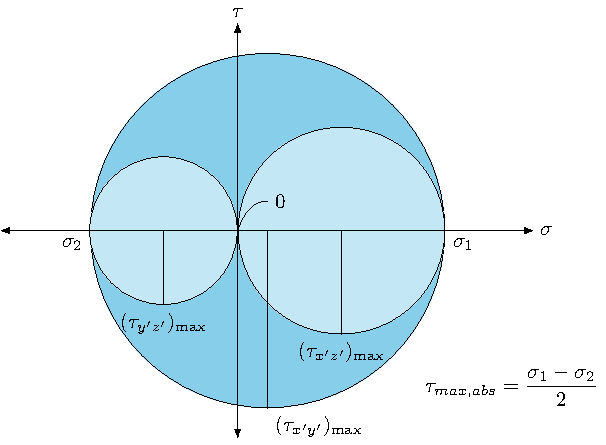
\includegraphics[width=.9\linewidth]{pictures/abs-max-shear-case-II.pdf}
\end{center}
\end{frame}

\begin{frame}[label={sec:org2021fa8}]{Example}
\begin{columns}
\begin{column}{0.5\columnwidth}
\begin{center}
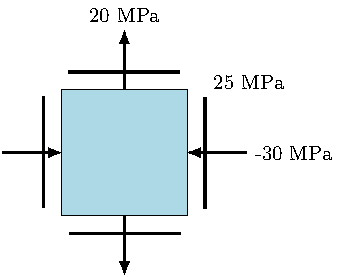
\includegraphics[width=.9\linewidth]{pictures/max-abs-shear-stress-problem.pdf}
\end{center}
\end{column}

\begin{column}{0.5\columnwidth}
\begin{itemize}
\item From previous example, we have that \(\sigma_1\) = 30.4 MPa,
\(\sigma_2\) = -40.4 MPa, and \(\tau_{\max}\) = 35.4 MPa.

\item Let us draw a Mohr's circle out of this.
\end{itemize}
\end{column}
\end{columns}
\end{frame}

\begin{frame}[label={sec:org2a9b95f}]{}
\begin{center}
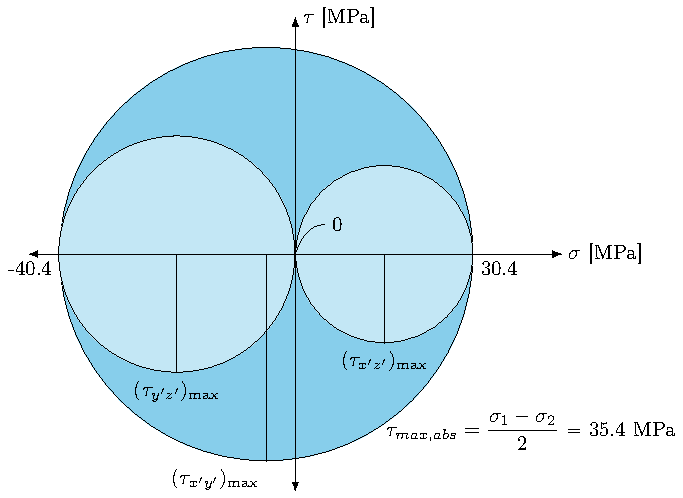
\includegraphics[width=.9\linewidth]{pictures/max-abs-shear-stress-example.pdf}
\end{center}
\end{frame}
\end{document}